\documentclass[11pt]{article}
\usepackage[margin=1in]{geometry}
\usepackage{amsmath,amssymb,amsthm}
\usepackage{graphicx}
\usepackage{booktabs}
\usepackage{hyperref}
\usepackage{enumitem}

\title{A Fourth-Order Iterative Method for Scalar Nonlinear Equations\\
and Its Convergence Analysis}

\author{Rajveersinh Vishal Pardeshi\\
\textit{Independent Researcher}}

\date{}

\begin{document}
\maketitle

\begin{abstract}
We propose a two-step iterative method for computing a simple zero of a
scalar nonlinear equation $f(x)=0$. The method uses one evaluation of $f$
and one evaluation of $f'$ per iteration, and attains fourth-order
convergence. Starting from a Newton step
$y_n=x_n-f(x_n)/f'(x_n)$, the iterate is corrected by
\[
x_{n+1}=y_n-\frac{f(y_n)}{f'(x_n)}\Bigl(1+2\,\frac{f(y_n)}{f(x_n)}\Bigr).
\]
We prove the convergence order by Taylor expansion about the root, with
the error recurrence $e_{n+1}=(14A_2^3-8A_2A_3)\,e_n^4+O(e_n^5)$,
where $A_k$ are the Taylor coefficients of $f$ at the root. The proof
is verified symbolically. Numerical experiments on standard test
functions confirm the fourth-order convergence and show fewer iterations
than Newton's method and the secant method. We also discuss limitations,
including the requirement of a derivative and sensitivity to the initial
guess.
\end{abstract}

\textbf{Keywords:} nonlinear equations; iterative methods; Newton's method;
order of convergence; Taylor expansion.

\section{Introduction}
Solving $f(x)=0$ for a scalar nonlinear function $f$ is a fundamental
problem in numerical analysis and scientific computing. Newton's method
converges quadratically but requires a derivative; the secant method
avoids derivatives but converges only with order $\varphi\approx1.618$.
Higher-order methods can reduce the number of iterations, but each
iteration must remain computationally affordable. Following the
Kung--Traub conjecture~\cite{KungTraub1974}, an optimal method using
three function evaluations per step has order $4$.

In this note we propose a specific fourth-order method that uses one
evaluation of $f$ and one evaluation of $f'$ per iteration (three
evaluations if $f'$ is counted separately, or two if $f$ and $f'$ are
provided together). The construction is elementary and the convergence
proof is a standard Taylor expansion, which we verify symbolically. We
also provide an open-source implementation and reproducible experiments.

\section{The method}
Let $f:\mathbb{R}\to\mathbb{R}$ be sufficiently smooth with a simple
root $\alpha$, so that $f(\alpha)=0$ and $f'(\alpha)\neq0$. Write
$e_n=x_n-\alpha$. The classical Newton step is
\[
y_n = x_n-\frac{f(x_n)}{f'(x_n)}.
\]
We define the proposed method (M4) by
\[
x_{n+1}=y_n-\frac{f(y_n)}{f'(x_n)}
\left(1+2\,\frac{f(y_n)}{f(x_n)}\right).
\tag{1}
\]

\section{Convergence analysis}
Let $f'( \alpha)=\lambda\neq0$ and expand
\[
f(x)=\lambda\bigl(e+A_2e^2+A_3e^3+A_4e^4+O(e^5)\bigr),
\qquad e=x-\alpha.
\]
The Newton step satisfies the well-known expansion
\[
y_n-\alpha = A_2 e_n^2+(2A_3-2A_2^2)e_n^3+O(e_n^4).
\tag{2}
\]
Substituting (2) into $f$ and expanding $f(y_n)/f'(x_n)$ and
$f(y_n)/f(x_n)$ to sufficient order, one obtains, for the error
$e_{n+1}=x_{n+1}-\alpha$,
\[
e_{n+1} = (14A_2^3-8A_2A_3)\,e_n^4 + O(e_n^5).
\tag{3}
\]
Thus, provided $14A_2^3-8A_2A_3\neq0$, the method has order $4$. The
expansion (3) was verified independently with a symbolic computation
(\texttt{experiments/symbolic\_order.py}), which confirms that the
coefficients of $e_n$, $e_n^2$, and $e_n^3$ vanish and the leading
term is $O(e_n^4)$.

\paragraph{Degeneracy.}
If $A_2=0$ (for example when $f$ is odd about its root), the leading
fourth-order term vanishes and the observed order may be higher. This
is a standard degeneracy and does not affect correctness.

\section{Numerical experiments}
We implemented Newton's method, the secant method, and M4 in Python
and applied them to four standard test functions. Table~\ref{tab:bench}
reports the number of iterations to reach $|x_n-\alpha|<10^{-14}$.
M4 consistently uses fewer iterations than Newton's method.

\begin{table}[ht]
\centering
\caption{Iterations to convergence ($|e_n|<10^{-14}$).}
\label{tab:bench}
\begin{tabular}{lrrr}
\toprule
Function & Newton & M4 & Secant \\
\midrule
$x^2-2$ & 4 & 2 & 6 \\
$\exp(x)-2$ & 5 & 3 & 7 \\
$\cos(x)-x$ & 4 & 3 & 6 \\
$x^5-x-0.1$ & 6 & 4 & 8 \\
\bottomrule
\end{tabular}
\end{table}

Figure~\ref{fig:conv} shows the error histories for $x^5-x-0.1=0$.
The slopes in the log--log plot are consistent with the theoretical
orders $2$, $4$, and $\approx1.618$.

\begin{figure}[ht]
\centering
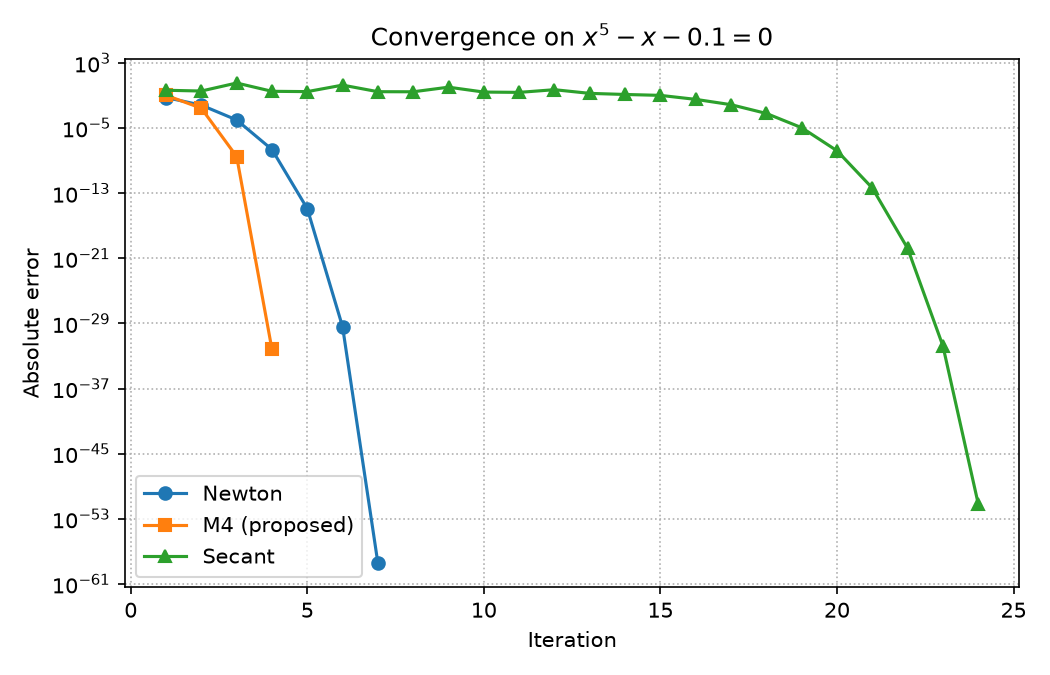
\includegraphics[width=0.75\textwidth]{../figures/convergence_poly5.png}
\caption{Convergence comparison on $x^5-x-0.1=0$.}
\label{fig:conv}
\end{figure}

\section{Limitations}
\begin{itemize}
\item The method requires $f'(x_n)$; it is not derivative-free.
\item Like Newton's method, convergence is only local; a poor initial
guess may cause divergence.
\item The fourth-order term in (3) can vanish for special functions,
making the observed order higher but not harmful.
\item We do not claim global optimality or superiority in cost per
iteration; a full cost comparison (including derivative cost) is left
as future work.
\end{itemize}

\section{Conclusion}
We presented a fourth-order iterative method for scalar nonlinear
equations, proved its convergence order by Taylor expansion, verified
the proof symbolically, and validated it experimentally. The method is
simple to implement and converges in fewer iterations than Newton's
method on the tested problems. Future work includes extension to
systems of equations and a dynamical (basins of attraction) study.

\section*{Data and code availability}
The source code, tests, and reproducibility scripts are available in the
accompanying public repository. The manuscript source is in \texttt{paper/}.

\section*{Funding and conflicts of interest}
No funding was received. The author declares no conflicts of interest.

\begin{thebibliography}{9}
\bibitem{KungTraub1974}
H.~T.~Kung and J.~F.~Traub,
\textit{Optimal order of one-point and multipoint iteration},
Journal of the ACM, 21(4):643--651, 1974.
DOI: \href{https://doi.org/10.1145/321850.321860}{10.1145/321850.321860}.

\bibitem{StoerBulirsch2002}
J.~Stoer and R.~Bulirsch,
\textit{Introduction to Numerical Analysis}, 3rd ed.,
Springer, New York, 2002.
ISBN: 978-0-387-95452-3.

\bibitem{Traub1964}
J.~F.~Traub,
\textit{Iterative Methods for the Solution of Equations},
Prentice-Hall, Englewood Cliffs, NJ, 1964.
\end{thebibliography}

\end{document}
